% !TeX document-id = {6a6080c6-c37a-4e47-968e-f57419892100}
% !TeX spellcheck = en_US
% !TeX encoding = UTF-8
% !TeX TXS-program:compile = txs:///latexmk/[-pdf -silent -shell-escape -interaction=nonstopmode -latexoption="-synctex=1" -output-directory="build"]
% !TeX TXS-program:quick = txs:///compile | txs:///view

\documentclass[a4paper,10pt,oneside]{article}

% -----Packages-----------------------------------------------------------------
\usepackage[german]{ethidscLab}
\usepackage{pstricks}
\usepackage{parskip}
\usepackage{latexsym}
\usepackage[ngerman]{cleveref}
\usepackage{subfig}
\usepackage{siunitx}

% -----Settings-----------------------------------------------------------------
\addtolength{\hoffset}{-1cm} \addtolength{\textwidth}{2cm}
\addtolength{\voffset}{-1.5cm} \addtolength{\textheight}{2.5cm}

\setlength{\parindent}{0pt}
\setlength{\parskip}\medskipamount

\tolerance 1000 \emergencystretch 1em \doublehyphendemerits 2500
\hfuzz 1pt \hbadness = 3000 \leftskip 0pt minus 1pt \rightskip 0pt
minus 1pt \interdisplaylinepenalty=2500

% -----Hypenation---------------------------------------------------------------
\hyphenation{Be-triebs-punkt ini-tia-li-sie-ren
Kreis-ver-star-kungs-dif-fe-renz Mess-la-bor}

% -----Title Page---------------------------------------------------------------
\lineone{Praktikum Mess- und Regeltechnik}
\linetwo{Anleitung zum Versuch}
\title{Air Massflow Sensor}
\authors{Christoph Bolli\\Daniel Matter\\André Niederberger\\Simon Wieser\\GianAndrea Müller}
\date{März 2019}

%-------------------------------------------------------------------------------
% -----Document-----------------------------------------------------------------
\begin{document}

\pagenumbering{alph}
\maketitle
\mbox{}
\thispagestyle{empty}
\newpage
\pagestyle{plain}
\pagenumbering{arabic}

\tableofcontents

\newpage

\section{Einleitung}
Heutige Emissionsgrenzwerte bei PKWs können nur durch Verwendung von Dreiweg-Katalysatoren erreicht werden. Diese funktionieren nur bei exakt stöchiometrischer Verbrennung, was heisst, dass genau die Menge Benzin eingespritzt werden muss, die mit dem vorhandenen Sauerstoff vollständig verbrennen kann. Um ein solches Gemisch zu erreichen, muss unter anderem der Luftmassenstrom im Saugrohr genau gemessen werden können, um die Einspritzmenge dementsprechend zu dosieren. In diesem Praktikum soll ein Prinzip aufgezeigt werden, mit dem eine solche Luftmassenstrommessung durchgeführt werden kann.

Ziele für den Studenten sind, die theoretischen Kenntnisse von den Grundvorlesungen Thermodynamik und Regelungstechnik kombiniert anwenden zu können. Ebenso soll vermittelt werden, dass sich die Realität weit weniger ideal verhält, als dies von theoretischen Übungen erwartet werden könnte.
Weiter soll ein erster Schritt im Umgang mit Ingenieurtools gemacht werden. In diesem Fall wird LabVIEW verwendet, welches ein in der Praxis weit verbreitetes Programm zur Messdatenerfassung ist.


%
\section{Thermodynamische Grundlagen}

\subsection{Funktionsprinzip}
Die Massenstrommessung beruht auf der Wärmekapazität der vorbeigeströmten Luft. Am Eingang der \textit{'Sonde'} wird die Temperatur erfasst ($\vartheta_1$), dann durchströmt die Luft ein Heizelement und am Ende wird die Temperatur wieder gemessen ($\vartheta_2$). Die Heizleistung wird so geregelt, dass der Temperaturunterschied zwischen den beiden Messstellen immer konstant ist. Unter der Voraussetzung, dass Luft im relevanten Bereich eine konstante Wärmekapazität hat, ist die Luftmassenmenge proportional zur Heizleistung. 

\begin{figure}[H]
\centering
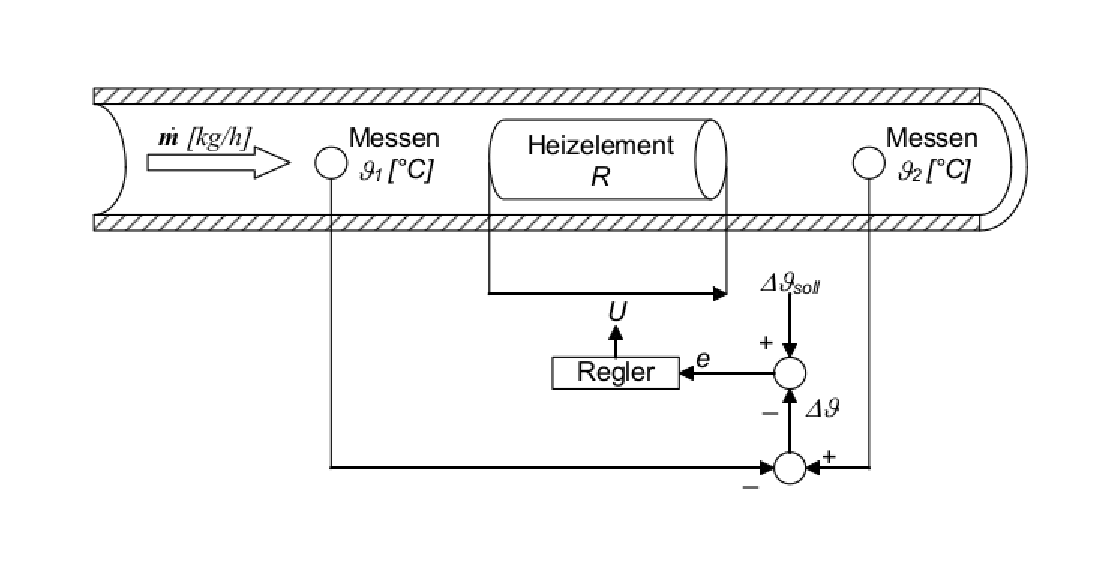
\includegraphics[width=\textwidth]{img/schema_luft.eps}
\caption{Schematischer Messaufbau}
\label{schemaaufbau}
\end{figure}
\newpage

\textbf{Aufgaben:} \\
Leiten Sie mit Hilfe von Abbildung \ref{schemaaufbau} die Abhängigkeit des Massenstroms von der angelegten Heizspannung und den Temperaturen $\vartheta_1$ und $\vartheta_2$ her!
Gehen Sie dabei folgendermassen vor:

\begin{enumerate}
\item Treffen Sie geeignete Annahmen, welche Ihnen die Arbeit erleichtern sollen.\\ \textit{Tipp:} Überlegen Sie sich, welche Energieflüsse vernachlässigbar sind!
\item Wenden Sie den 1. Hauptsatz der Thermodynamik an, indem Sie über ein von Ihnen bestimmtes Kontrollgebiet die Energiebilanz aufstellen.\\ \textit{Tipp:} Drei Energieströme sind zu berücksichtigen!
\item Lösen Sie die erhaltenen Gleichungen nach dem Massenstrom auf!\\ \textit{Tipp:} Nehmen Sie statisches Verhalten an!\\
\end{enumerate}


\textbf{Lösungen zu Aufgaben:}

\begin{enumerate}
\item \begin{itemize} \item Da die Luft nur um einige Grad erhitzt wird, kann sie als perfektes Gas angenommen werden. \item Die potentielle und die kinetische Energie der Luft kann vernachlässigt werden. \item Die Wärmeleitung durch die Wand kann bei grossen Temperaturen einen gewissen Einfluss haben, einfachheitshalber wird sie hier aber vernahlässigt. \item Das Temperaturprofil innerhalb der Röhre soll bei beiden Temperaturfühlern konstant sein. \item Sämtliche Überlegungen gelten bei stationärem Betrieb. \end{itemize}
\item Das Kontrolgebiet wird um das Heizelement gelegt, mit den Grenzen auf den Temperaturfühlern.
\end{enumerate}

\begin{figure}[H]
\centering
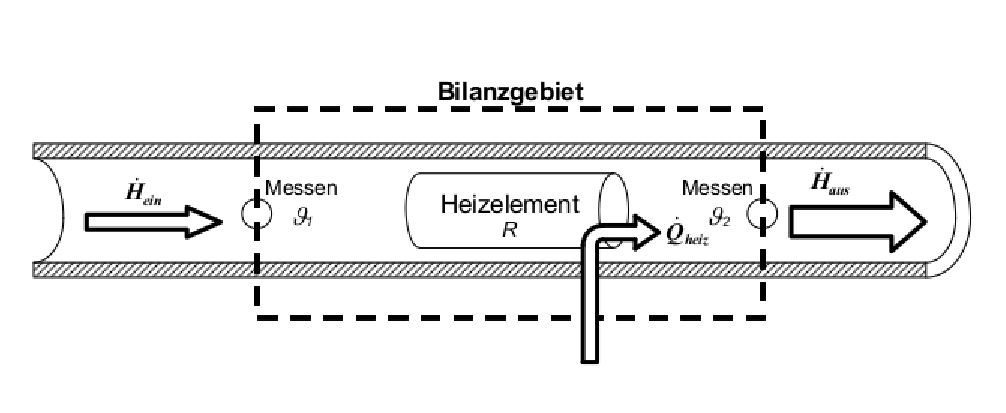
\includegraphics[width=\textwidth]{img/kontrollgebiet.eps}
\caption{Kontrollgebiet und Energieströme}
\label{kontrollgebiet}
\end{figure}

Der erste Hauptsatz über das Kontrollgebiet lautet:
\begin{equation}\label{eqn_haupt}
\dot{H}_{aus}=\dot{H}_{ein}+\dot{Q}_{heiz}
\end{equation}


Mit $c_p$ als Wärmekapazität der Luft, beträgt der Enthalpiestrom der einströmenden Masse:
\begin{equation}\label{eqn_ein}
\dot{H}_{ein}=\dot{m }\cdot c_p \cdot \vartheta_1
\end{equation}


Analog dazu beträgt der Enthalpiestrom der ausströmenden Masse:
\begin{equation}\label{eqn_aus}
\dot{H}_{aus}=\dot{m} \cdot c_p \cdot \vartheta_2
\end{equation}


Die Heizleistung des Widerstandes beträgt:
\begin{equation} \label{eqn_leistung}
\dot{Q}_{heiz}=P=U \cdot I = \frac{1}{R} \cdot U^2
\end{equation}


Durch einsetzen von \eqref{eqn_ein}, \eqref{eqn_aus} und \eqref{eqn_leistung} in \eqref{eqn_haupt} ergibt:
\begin{equation}
\dot{m} \cdot c_p \cdot \vartheta_2=\dot{m} \cdot c_p \cdot \vartheta_1+P
\end{equation}


Aufgelöst nach dem Massenstrom $\dot{m}$ ergibt sich:
\begin{equation}
\dot{m}=\frac{P}{\left(\vartheta_2 - \vartheta_1 \right) \cdot c_p}
\end{equation}


Wird nun die Spannung über dem Heizwiderstand so geregelt, dass die gemessene Temperaturdifferenz konstant ist, so ist der Luftmassenstrom linear in $P$ (resp. in $U^2$, wenn $R$ als konstant angenommen wird) und kann somit einfach bestimmt werden.


\section{Regeltechnische Grundlagen}

Allgemein gehen wir in der Regelungstechnik von einer Regelstrecke aus, in der wir mit einer Stellgrösse, die wir beeinflussen können, eine Regelgrösse auf einem bestimmten Wert halten wollen.

\begin{figure}[H]
\centering
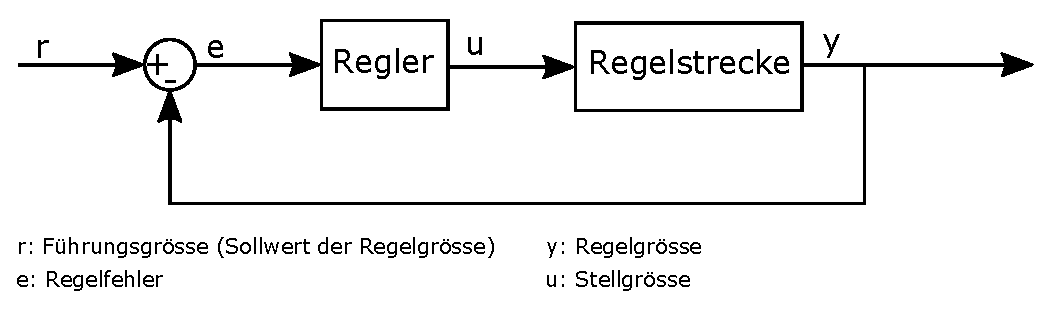
\includegraphics[width=0.8\textwidth]{img/regelkreis.eps}
\caption{Grundstruktur Regelkreis}
\label{regelkreis}
\end{figure}


Die Regelgrösse y wird abgegriffen und mit dem Sollwert r, welcher auch zeitvariant sein kann, verglichen. Auf Grund dieser Differenz, dem Regelfehler e, berechnet der Regler nun die Stellgrösse u, welche in der Strecke wieder eine korrekte Regelgrösse bewirken soll.

\subsection{Der P-Regler}
Der Regler stellt einen Zusammenhang zwischen dem Regelfehler und der Stellgrösse her. Es ist naheliegend, diesen Zusammenhang linear zu gestalten. Das heisst, je grösser der Regelfehler ist, desto grösser soll auch die Stellgrösse werden.

\begin{equation}
\Delta u = K_r \cdot e
\end{equation}

mit $K_r$ statischer Übertragungsfaktor (Regel-Verstärkung)

Da die Stellgrösse beim Betriebspunkt einen gewissen Wert haben soll, muss dem Regelalgorithmus noch ein konstantes Glied angehängt werden.

\begin{equation}
u = K_r \cdot e + A
\end{equation}

A: Stellgrösse bei $e=0$ (Aufrechterhalten des gewünschten Betriebspunktes, Vorsteuerung)

Dieser Regler wird P-Regler genannt, da das Korrektursignal zum Regelfehler proportional ist.

Je grösser $K_r$ ist, desto stärker wird der Regelfehler auskorrigiert. Dadurch erreicht aber der Reglerausgang schneller die Sättigungsgrenze. Weiter besteht die Gefahr von Instabilität, da die Strecke immer gewisse Modellierungsfehler enthält.

\textbf{Da ein P-Regler nur arbeiten kann, wenn ein Regelfehler vorhanden ist, kann eine Abweichung in der Regelgrösse nie ganz weggeregelt werden, es bleibt immer ein gewisser Regelfehler zurück.}

\subsection{Der PI- und der PID-Regler}
Nimmt man den bleibenden Regelfehler und integriert ihn in jedem Zeitschritt auf, so erhält man ein Mass für die bleibende zeitliche Abweichung des Regelfehlers, welches seinen Wert ändert, solange der Regelfehler nicht null ist. 
Es wird eine Zeitkonstante festgelegt, wie schnell der aufintegrierte Teil ausgeregelt werden soll.

\begin{equation}
u= K_R \cdot e + \frac{K_R}{T_N} \int_{0}^{t} e(\tau)d\tau + A(t=0)
\end{equation}

$T_N$: Nachstellzeit

Da sich der Regler jetzt selbst auf einen neuen Betriebspunkt einstellen kann, ist die Angabe des Betriebspunktes A nicht mehr zwingend notwendig.

Dieser Regler wird PI-Regler genannt, da er einen proportionalen und einen integralen Teil aufweist.

Die vom P-Anteil zurückbleibende Regeldifferenz wird um so schneller abgebaut, je kleiner die Nachstellzeit TN gewählt wird. Sie gibt die Zeit an, bei der das Ausgangssignal des I-Reglers bei konstantem Fehlersignal gleichgross ist wie dasjenige des P-Reglers. Bei zu schnellem Abbau tritt wiederum schwingendes Verhalten auf: Bei zu schnellem Nachstellen des Arbeitspunktes kann dieser über das Ziel \grqq hinausschiessen\grqq  \,(Eine Änderung des Arbeitspunktes wirkt sich verzögert auf die Regelgrösse und damit auf den Regelfehler aus). Ein Zurückschieben des Arbeitspunktes kann aber erst erfolgen, wenn die Regeldifferenz das Vorzeichen wechselt, d.h. wenn die Regelgrösse den Sollwert über- oder unterschreitet. Dadurch wird die Schwingneigung gefördert. Der I-Regler hat im Bode-Diagramm 90° Phasenverlust (d.h. er ?hinkt? hinterher). Das ist der Grund, warum der Regelkreis instabiler wird. 

Um die transiente Antwort zu beschleunigen, wird ein D-Anteil eingeführt. Das hat den Vorteil, dass 90° Phase gewonnen werden, was die Stabilität verbessert. $T_V$ ist die Vorhaltezeit, bei der das Ausgangssignal des D-Reglers bei rampenförmigem Fehlersignal gleichgross ist wie dasjenige des P-Reglers.

\begin{equation}
u= K_R \cdot e + \frac{K_R}{T_N} \int_{0}^{t} e(\tau)d\tau + K_R \cdot T_V \frac{de(\tau)}{d\tau} \, \left[+ A(t=0)\right]
\end{equation}

Zusammenfassend könnte man sagen, dass der P-Anteil sich die Gegenwart interessiert, der I-Anteil für die Vergangenheit und der D-Anteil für die Zukunft.



\subsection{Klassische Einstellregeln von Ziegler-Nichols}\label{ZN}

Das Einstellen der PID-Regelparameter kann auf verschiedene Weisen erfolgen. Nicht immer ist ein Einstellen \glqq von Auge\grqq \, möglich, wo Parameter sukzessive verändert werden, bis das Resultat den Ansprüchen genügt. 

Die Einstellregeln von Ziegler-Nichols sind eine Variante, wie Regelparameter schnell und einfach eingestellt werden können. Dieses Verfahren ist in der Industrie beliebt, weil vom System kein Modell erarbeitet werden muss.

Vorgehen:
\begin{itemize}
\item Der Regler wird als reiner P-Regler geschaltet;
\item Einschwingvorgang anregen durch Sprung in Führungs- oder Störgrössen;
\item Durch Veränderung von $K_R$ die Stabilitätsgrenze suchen.
\item Kennwerte bestimmen:
\begin{itemize}
\item $K_{R_{krit}}$ = Verstärkung $K_R$, bei der eine grenzstabile Dauerschwingung entsteht
\item $T_{krit}$ = Periodendauer der grenzstabilen Dauerschwingung
\end{itemize}
\item Nach Ziegler-Nichols die Reglerparameter für die gewünschte Reglerstruktur bestimmen
\end{itemize}

\begin{center}
\begin{tabular}{|l| l  c l|}
\hline
P-Regler & $K_R$ &  = & $ 0.5 \cdot K_{R_{krit}}$ \\ \hline\hline
\multirow{2}{*}{PI-Regler} &  $K_R$ &  = & $ 0.45 \cdot K_{R_{krit}}$ \\ \cline{2-4}
 & $T_N$ & = & $0.85 \cdot T_{krit}$ \\ \hline\hline
\multirow{3}{*}{PID-Regler} & $K_R$ &  = & $ 0.6 \cdot K_{R_{krit}}$ \\ \cline{2-4}
 &  $K_R$ &  = & $ 0.5 \cdot T_{krit}$ \\ \cline{2-4}
  & $T_V$ & = & $0.125 \cdot T_{krit}$ \\ \hline
\end{tabular}
\end{center}


\subsection{Nichtlineare Einstellregeln von Ziegler-Nichols}

Das oben beschriebene Vorgehen birgt für gewisse Systeme Risiken. Sollte zum Beispiel für ein Flugzeug ein Höhenregler gebaut werden, müsste das Flugzeug \textit{fast} instabil gemacht werden, was nicht alle Passagiere, die dem Versuch beiwohnen, erfreuen würde. Gleiches wenn ein Atomkraftwerk \textit{fast} instabil werden soll.

Die Lösung zu diesem Problem ist, wenn man den P-Regler durch einen Nichtlinearen-Zwei-Punkt-Regler ersetzt. Dieser Regler gibt bei positiven Fehlerwerten einen konstanten Wert $d$ als Stellgrösse aus, und bei negativen Fehlern den Wert $-d$. Dieser nichtlineare Regler führt zu einem Schwingen des Regelkreises mit (begrenzter) Amplitude $a_c$  und Periode $T_{krit}$ (gleich $T_c$). 


\begin{figure}[H]
\centering
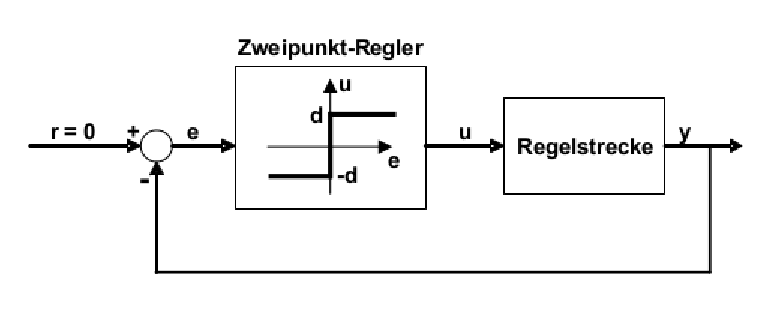
\includegraphics[width=10cm]{img/zweipunkt.eps}
\caption{Zweipunkt-Regler}
\label{2punkt}
\end{figure}


\begin{figure}[H]
\centering
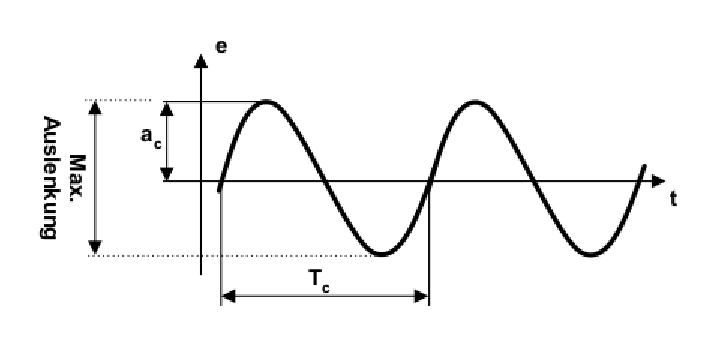
\includegraphics[width= 10cm]{img/amplitude.eps}
\caption{Amplitude des Regelkreises}
\label{ampli}
\end{figure}

Daraus kann mittels nichtlinearer Regeltheorie (Methode der ersten harmonischen) die kritische Verstärkung berechnet werden:

\begin{equation}
K_{R_{krit}}=\frac{4\cdot d}{\pi \cdot a_c}
\end{equation}

Mit diesen Werten können nun in der bekannten Tabelle von Ziegler/Nichols die Einstellwerte nachgeschlagen werden.

Die Amplitude $a_c$ kann auch als die Hälfte der maximalen Auslenkung (in beide Richtungen) des Fehlersignals bestimmt werden.
Die so gefundenen Reglereinstellungen müssen nicht die optimalen sein, sie bilden aber eine gute Grundlage, um noch bessere Parameter finden zu können.

\textbf{Aufgaben:}

Legen Sie die Eingangs- und Ausgangsgrössen des Luftmassenstrommessers fest. Überlegen Sie sich, wo die Führungsgrösse, Regelgrösse, Stellgrösse und der Regelfehler auftritt.


\textbf{Lösung zu den Aufgaben} 

Eingangsgrösse der Regelstrecke ist die Spannung U, die am Heizelement angelegt wird. Ausgangsgrössen sind die zwei gemessenen Temperaturen $\vartheta_1$ und $\vartheta_2$. Die Führungsgrösse entspricht der Solltemperaturdifferenz $\Delta\vartheta_{soll}$ und ist im Fall des Luftmassenstrommessers konstant. Stellgrösse ist die Spannung $U$. Regelgrösse ist die Temperaturdifferenz $\vartheta_2-\vartheta_1$, wobei nur die Differenz interessiert und nicht die absoluten Werte. Der Regelfehler entspricht der Differenz zwischen Führungsgrösse und Regelgrösse, also $\Delta\vartheta_{soll}-(\vartheta_2-\vartheta_1 )$.

\newpage


\section{System kennen lernen}

Betrachten sie nun das System und identifizieren sie die verschiedenen Komponenten. Zusätzlich zum selbstgebauten Massenstrommesser sind im Versuchsaufbau auch eingebaut:
\begin{itemize}
\item Ein serienmässiger Massenstrommesser, wie er in Automobilen eingesetzt wird, um die gemessenen Resultate zu beurteilen.
\item Eine Drosselklappe, welche ermöglicht, vom Computer aus den Massenstrom zu verändern.
\item Verschiedene strömungstechnische Einrichtungen, welche die Strömung führen und beruhigen sollen.
\end{itemize}

Nehmen Sie jetzt den Massenstrommesser in Betrieb:
LabVIEW wird automatisch gestartet und die Anwendungsdatei wird geöffnet. (Ansonsten öffnen Sie die Datei unter C:\textbackslash thermotronic\textbackslash thermotronic.vi in LabVIEW)
Das Panel zur Bedienung der Einrichtung erscheint. Betrachten Sie das Panel und identifizieren Sie die verschiedenen Elemente. Sämtliche Drehknöpfe und Schalter können mit der Maus eingestellt werden\footnote{Zum Verstellen der Werte muss der Mauszeiger als Hand erscheinen, ist dies nicht der Fall, drücken Sie die Tabulatortaste, bis der Mauszeiger eine Hand wird}.

\subsection{System starten}
Um das System zu starten, arbeiten Sie folgende Punkte durch:
\begin{itemize}
\item Bevor Sie das Programm starten, stellen Sie sicher, dass:
\begin{itemize}
\item die Frosselklappe geöffnet ist. $(90^\circ)$
\item der Modus \glqq manuell\grqq \, ist.
\item die Sollleistung bei Betrieb ohne Regler 0\% ist.
\end{itemize}

\item Starten Sie jetzt das Programm durch klicken auf 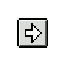
\includegraphics{img/arrow.eps} in der Symbolleiste:

\item Schalten Sie die Elektronik ein (Schalter an der Hinterseite);

\item Schalten Sie den Staubsauger ein.

\end{itemize}


\section{Regler auslegen und in Betrieb setzen}

\subsection{Modus \glqq Manuell\grqq}

Sie sind vorerst der Regler!

Versuchen Sie mit dem Drehschalter für die Sollleistung von Hand die geforderten $6^\circ C$ Temperaturdifferenz einzustellen. Versuchen sie einen Drosselklappensprung so schnell als möglich auszuregeln. 

\newpage
\subsection{Modus \glqq PID-Einstellregeln klassisch nach Ziegler-Nichols\grqq}

Legen Sie einen P-, PI und PID-Regler für das Heizelement des Luftmassenstrommessers aus. Gehen Sie dabei so vor, wie in \ref{ZN} beschrieben wurde. 

Suchen Sie die kritische Verstärkung eines reinen P-Reglers in wenigstens zwei verschiedenen Arbeitspunkten!
In realen Systemen sind keine unendlich grosse Schwingungen möglich. Begründen Sie, warum das so ist!
Sie beobachten bei überkritischen Verstärkungen des P-Reglers, dass wachsende Schwingungsamplituden begrenzt werden. Somit stellt sich auch bei überkritischer Verstärkung eine grenzstabile Schwingung ein. Beobachten Sie also das Regelsystem, wenn keine Begrenzungen das Verhalten beeinflussen! Es ist schwierig, die kritische Verstärkung direkt zu finden. Einfacher finden Sie einen Verstärkungsfaktor, der knapp aber eindeutig überkritisch ist, sowie einen Verstärkungsfaktor, der knapp und eindeutig stabil ist. Berechnen Sie aus dem Mittelwert dieser zwei Faktoren die kritische Verstärkung!

Mit Hilfe des Regelfehler-Diagrammes können Sie die Periodendauer $T_{krit}$ bestimmen. Wenn Sie das Programm mit der STOP-Taste unterbrechen, können Sie die Zeit bequem ablesen. Anschliessend können Sie das Programm mit der 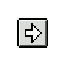
\includegraphics{img/arrow.eps} Taste neu starten.

Berechnen Sie die Regelparameter für die gewünschte Reglerstruktur nach Ziegler-Nichols und stellen Sie die entsprechenden Werte im Modus \glqq Regler\grqq ein!

\subsection{Modus \glqq Einstellregeln nichtlinear nach Ziegler-Nichols\grqq}
Wählen Sie den Modus \grqq Ziegler-Nichols-Nichtlinear\grqq. Weiter können Sie die Begrenzung des Zweipunktreglers $d$ einstellen. In unserem Fall kann $d$ nicht grösser als $5V$ gewählt werden, da sonst die Heizspirale in eine Sättigung hineinläuft. Bestimmen Sie die Amplitude $a_c$ und die Periode $T_c$. Die Amplitude $a_c$ kann auch als die Hälfte der maximalen Auslenkung (in beide Richtungen) des Fehlersignals bestimmt werden.

\begin{itemize}
\item Probieren Sie verschiedene Werte von $d$ aus. Was passiert mit der jeweiligen Amplitude $a_c$ des Fehlersignals? Wie verändern sich $K_R$, $T_{krit}$?
\item Berechnen Sie die Regelparameter nach Ziegler-Nichols und stellen Sie die entsprechenden Werte wie    im Modus \glqq Regler\grqq ein!
\end{itemize}


\subsection{PID-Regler}

Was haben die verschiedenen Anteile des PID-Reglers für einen Einfluss auf den Regelfehler? Schalten Sie die einzelnen Anteile des PID-Reglers ein und aus. Dabei ändert sich die Reglerstruktur und es müssen neue Werte nach Ziegler-Nichols berechnet werden.

\begin{itemize}
\item Was ändert sich an der Glätte des Fehlersignals wenn der D-Anteil aktiviert wird? Siehe dazu die Bemerkungen zum PID-Regler in Kapitel 11.2.1 im Buch Analysis and Synthesis of Single-Input Single-Output Control Systems.
\end{itemize}

Versuchen Sie von Hand die erhaltenen Regelparameter zu verbessern. Erläutern Sie dabei, wie Sie vorgehen!

\newpage
\section{Fehlerabschätzung}
Notieren Sie Messwerte des Massenstrom-Sensors von der Firma Bosch und des selbstgebauten Sensores bei einigen Drosselklappenstellungen. Schalten Sie nun zuerst die Elektronik aus, dann den Staubsauger. 
Wie Sie bemerkt haben, ist die Massenstrommessung mit der selbstgebauten Einrichtung viel langsamer als mit dem von Bosch gelieferten Heissfilmmesser, obwohl dieser ähnlich funktioniert.


\textbf{Aufgaben:}
\begin{enumerate}
\item Nennen Sie verschiedene Elemente unserer Einrichtung, welche dazu beitragen, dass die Messung im Vergleich zum Bosch Sensor langsamer wird. Geben Sie Verbesserungsvorschläge!
\end{enumerate}

Wenn wir davon ausgehen, dass der Massenstrom-Sensor der Firma Bosch genau misst, sind neben den Verzögerungen der Versuchs-Einrichtung auch bleibende Fehler zu erkennen.


\textbf{Aufgaben:}
\begin{enumerate}
\setcounter{enumi}{1}
\item Kontrollieren Sie die nachfolgende Überprüfung der Annahme eines isobaren Überganges. Ist das gewählte Modell realistisch?

\begin{equation}
\Delta p=\rho\lambda\frac{L}{D}\frac{\bar{u}^2}{2}
\end{equation}

\begin{tabular}{l@{$\quad$}l}
Rohrinnendurchmesser&$D = \SI{40}{\milli\meter}$\\
Rohrlänge&$L=\SI{170}{\milli\meter}$\\
Rauhigkeitstiefe&$k_s=\SI{0.0015}{\milli\meter}$\\
Mittlere Fliessgeschwindigkeit&$\bar{u}=\frac{\tilde{\dot{m}} R_L T_1}{A p_N}\approx\SI{16}{\meter\per\second}$\\
$\quad$Fehlerbehafteter Massenfluss&$\quad\tilde{\dot{m}}=\SI{85}{\kilo\gram\per\hour}$\\
$\quad$Gaskonstante für Luft&$\quad R_L=\SI{287.085}{\joule\per\kilo\gram\per\kelvin}$\\
$\quad$Temperatur an Sonde 1&$\quad T_1=\SI{300}{\kelvin}$\\
$\quad$Normdruck&$\quad p_N=\SI{101325}{\pascal}$\\
\\
Reynoldszahl&$Re_D=\frac{\bar{u}D_{red}}{\nu}\approx\SI{43000}{}$\\
$\quad$Kinematische Viskosität von Luft&$\quad\nu=\SI{14.9e-6}{\meter\squared\per\second}$\\
Rohrreibungszahl (Moody)&$\lambda=\SI{0.023}{}\quad @\frac{k_s}{D_{red}}=\SI{3.75e-5}{}$\\
\\
Dichte von Luft&$\rho=\frac{p_N}{R_LT_1}=\SI{1.176}{\kilo\gram\per\meter\cubed}$
\end{tabular}

\vspace{1.5ex}

\[\Delta p=\SI{1.176}{\kilo\gram\per\meter\cubed}\cdot 0.023\cdot\frac{\SI{170}{\milli\meter}}{\SI{40}{\milli\meter}}\cdot\frac{(\SI{16}{\meter\per\second})^2}{2}\approx\SI{15}{\pascal}\]

Das ist eine relative Abweichung vom Normdruck von $\frac{\Delta p}{p_N}\approx 0.015\%$.

\item Überlegen Sie sich im Folgenden welche weiteren Annahmen verletzt wurden.
\item Nutzen sie die unten gegebenen Fehlerwerte um basierend auf den Grundregeln der Fehlerrechnung eine Abschätzung des totalen Fehlers des geschätzten Massenstromes zu machen.
\end{enumerate}


\begin{itemize}
\item Fehler in der Leistungsmessung
\begin{enumerate}
\item Der Fehler der Leistungsrückmeldung beträgt 3\%.
\item Wandwärmeverluste betragen 5\%.
\item Weitere Faktoren $\rule{8cm}{0.15mm}$
 
Für die weitere Rechnung werden $3.5\%$ angenommen.
\end{enumerate}

Somit wird der gesamte relative Fehler der Leistungsmessung vereinfacht berechnet als:

\begin{equation*}
\frac{\delta P}{|P|} = 11.5\%
\end{equation*}

\item Fehler in der Temperaturmessung
\begin{enumerate}
\item Der erste Temperaturfühler sind mit einem Fehler von $\SI{0.1}{\celsius}$ behaftet.

\begin{equation*}
\delta T_1 = \SI{0.1}{\celsius}
\end{equation*}
\item Die Temperatur beim zweiten Messfühlers kann zusätzlich wegen der nicht gleichmässigen Temperaturverteilung im Rohr nur auf 5\% der Temperaturdifferenz bestimmt werden.
\begin{equation*}
\delta T_2 = \rule{5cm}{0.15mm} \SI{}{\celsius}
\end{equation*}
\end{enumerate}

Wenden Sie die Grundregeln der Fehlerberechnung an um den gesamten Fehler in der Temperaturmessung zu bestimmen:

\begin{equation*}
\delta \Delta T = \rule{5cm}{0.15mm}\SI{}{\celsius}
\end{equation*}
\end{itemize}

Berechnen Sie nun den gesamten relativen Fehler des Massenstroms:

\begin{equation*}
\frac{\delta\tilde{\dot{m}}}{|\tilde{\dot{m}}|} = \rule{10cm}{0.15mm}
\end{equation*}

Beurteilen Sie nun, ob die gemessenen Resultate im erwarteten Bereich liegen.

\section{Grundregeln der Fehlerrechnung}

Wenn Q eine Kombination von Summen und Differenzen ist:

\begin{equation*}
Q = a+b+\cdots+c-(x+y+\cdots+z),
\end{equation*}

dann

\begin{equation}
\delta Q = \sqrt{(\delta a)^2+(\delta b)^2+\cdots+(\delta c)^2+(\delta x)^2+(\delta y)^2+\cdots+(\delta z)^2}.
\end{equation}

Wenn Q eine Kombination von Multiplikationen und Divisionen ist:

\begin{equation*}
Q=\frac{ab\cdots c}{xy\cdots z},
\end{equation*}

dann

\begin{equation}
\frac{\delta Q}{|Q|}=\sqrt{\left(\frac{\delta a}{a}\right)^2+\left(\frac{\delta b}{b}\right)^2+\cdots+\left(\frac{\delta c}{c}\right)^2+\left(\frac{\delta x}{x}\right)^2+\left(\frac{\delta y}{y}\right)^2+\cdots+\left(\frac{\delta z}{z}\right)^2}.
\end{equation}
























\end{document}
